\chapter{Opis projektnog zadatka}
		
		\textbf{\textit{dio 1. revizije}}\\
		
		\textit{Na osnovi projektnog zadatka detaljno opisati korisničke zahtjeve. Što jasnije opisati cilj projektnog zadatka, razraditi problematiku zadatka, dodati nove aspekte problema i potencijalnih rješenja. Očekuje se minimalno 3, a poželjno 4-5 stranica opisa.	Teme koje treba dodatno razraditi u ovom poglavlju su:}
		\begin{packed_item}
			\item \textit{potencijalna korist ovog projekta}
			\item \textit{postojeća slična rješenja (istražiti i ukratko opisati razlike u odnosu na zadani zadatak). Dodajte slike koja predočavaju slična rješenja.}
			\item \textit{skup korisnika koji bi mogao biti zainteresiran za ostvareno rješenje.}
			\item \textit{mogućnost prilagodbe rješenja }
			\item \textit{opseg projektnog zadatka}
			\item \textit{moguće nadogradnje projektnog zadatka}
		\end{packed_item}
		
		\textit{Za pomoć pogledati reference navedene u poglavlju „Popis literature“, a po potrebi konzultirati sadržaj na internetu koji nudi dobre smjernice u tom pogledu.}
		\eject
		
		Potreba za kvalitetnom digitalizacijom bankarskih procesa i uvid u stanje pojedinih računa iz udobnosti doma od velikog su značaja kako za klijente, tako i za djelatnike banke. Cilj je ovog projekta razviti bankarski sustav: bazu podataka i sučelja prema bankarima, administratorima te krajnjim korisnicima banke, odnosno građanima.
		Korisnike dijelimo u nekoliko skupina : 
		\begin{packed_item}
			\item \textbf{administratori}, 
			\item \textbf{bankari},
			\item \textbf{službenici za odobravanje kreditnih zahtjeva građana} i 
			\item \textbf{korisnici u užem smislu} (građani).
		\end{packed_item}
		
		Svaka vrsta korisnika sustava ima svoj jedinstveni pogled u sustav putem web sučelja i Android aplikacije.
		
		\textit{\textbf{Neregistrirani korisnik}}, za registraciju u sustav upisuje svoj OIB i jedinstveni ključ koji je dobio od bankara. Nakon uspješnog unosa tih podataka, odabire korisničko ime i lozinku koji će mu u buduće služiti za prijavu u sustav. Ostale podatke o pojedinom korisniku kao što su: ime, prezime, adresa prebivališta, datum rođenja, e-mail adresa, sliku korisnika i dr., u sustav unosi bankarski službenik prilikom ugovaranja bilo kakve usluge banke.
		
		\textit{\textbf{Administrator}} u sustav ulazi putem unaprijed definirane web adrese gdje unosi svoje korisničko ime i lozinku koji mu daju pristup sustavu. On vidi popis svih korisnika sustava te može uređivati podatke za bilo koju vrstu korisnika, kao i dodavati te brisati same korisnike sustava. Jedina je osoba koja može kreirati račune ostalim djelatnicima banke.
		
		\textit{\textbf{Bankar}} svoj korisnički račun dobivaju od administratora. Ime, prezime, adresa prebivališta, OIB, datum rođenja, e-mail adresa i slika profila unaprijed su poznati podaci koje u sustav unosi administrator za svakog novog djelatnika. Pošto postanu dio kolektiva banke te nakon što administrator unese njihove podatke u sustav, u web aplikaciju unose svoj OIB i datum rođenja te tako dobivaju mogućnost odabira korisničkog imena i lozinke. U sustavu imaju uvid u sve svoje osobne podatke, ali nemaju mogućnost izmjene tih podataka.
		Bankar nema uvid u popis korisnika sustava, niti u popis klijenata banke (građana). On može otvoriti, obrisati ili mijenjati profile klijenata. Kako bi pronašao profil nekog građana i uređivao ga ili brisao, dužan je unijeti OIB osobe za koju radi izmjenu u sustavu nakon čega mu se otvara profil te osobe. Također mu je dozvoljeno otvarati i zatvarati tekuće, žiro, štedne račune, ugovarati kredite, kreditne i debitne kartice za korisnike banke, aktivacija i deaktivacija kartica te obavljanje transakcija po računima klijenata.
		
		Svaki tekući račun ima dozvoljeno prekoračenje, a svaka kreditna kartica ima ugovoren limit.
		
		\textit{\textbf{Klijent}} dobiva dozvolu pristupa sustavu od bankara. Klijent banke ima uvid u sve podatke o svom profilu (ime, prezime, OIB, prebivalište, datum rođenja, slika profila i drugo), ali ih ne može mijenjati. Također, klijent može vidjeti sve svoje transakcijske račune, štedne račune, ugovorene kredite i kartice (debitne i kreditne). Klijent ne može mijenjati osobne podatke, podatke o računima, kreditima ili karticama. Klijent može vršiti prijenos sredstava između svojih računa transakcijskih računa (tekućeg, žiro ili štednog) ili na račune drugih klijenata banke. Također, klijent može ručno izvršiti uplatu kredit ili na kreditnu karticu kako bi umanjio iznos dugovanja ili otplatiti dugovanje ukupno.
		
		Svi korisnici moraju imati sliku profila (standardna slika za osobnu iskaznicu).
		
		Jednom mjesečno, u web aplikaciji, korisniku dolazi izvod po svim transakcijskim računima i kreditnim karticama u PDF i XLS obliku.
		
		Također, potrebno je da banka ima definirane poslovnice. Svaka poslovnica u sustavu ima ime poslovnice, adresu poslovnice i jedinstveni identifikator. Svaki djelatnik banke vezan je za jednu od poslovnica. Dodatno, svaki klijent može zatražiti sastanak u određenoj poslovnici u određeno vrijeme u budućnosti kojeg preuzima neki od slobodnih bankara te poslovnice. Nakon što bankar odobri sastanak, klijentu u web sučelje dolazi obavijest u kojoj je navedeno ime poslovnice, adresa poslovnice, ime bankara te datum i vrijeme zakazanog sastanka.
		
		\textit{\textbf{Službenici za odobravanje kreditnih zahtjeva građana}} imaju uvid u svoje osobne podatke koje ne mogu mijenjati. Također, vidljivi su im svi neobrađeni kreditni zahtjevi svih klijenata banke. Službenik može preuzeti bilo koji zahtjev na obradu te tada ima uvid u podatke o zahtjevu i sve podatke o klijentu koje banka posjeduje. Podaci o zahtjevu mogu biti iznos zatraženog kredita, namjena kredita, kamatna stopa i vrijeme otplate ako se radi o zahtjevu za kredit, odnosno vrsta zaražene kreditne kartice ako se radi o zahtjevu za kreditnom karticom. Službenik tada odobrava ili odbija zahtjev za kreditom, odnosno odobrava ili odbija kreditnu karticu s određenim limitom i kamatnom stopom.
		Nakon donesene odluke, korisnik tu odluku vidi u aplikaciji.
		
		Rate za kredite i kreditne kartice klijenata skidaju se automatski svaki mjesec na datum kojeg odredi administrator sustava i on je jedinstven za sve. U slučaju da na tekućem računu korisnika ne postoji dovoljno sredstava, ta se rata odgađa za jedan mjesec i bit će naplaćena zajedno s novom ratom idući mjesec.
		\eject
		
		\section{Primjeri u LaTeXu}
		
		\textit{Ovo potpoglavlje izbrisati.}\\

		U nastavku se nalaze različiti primjeri kako koristiti osnovne funkcionalnosti LaTeXa koje su potrebne za izradu dokumentacije. Za dodatnu pomoć obratiti se asistentu na projektu ili potražiti upute na sljedećim web sjedištima:
		\begin{itemize}
			\item Upute za izradu diplomskog rada u LaTeXu - \url{https://www.fer.unizg.hr/_download/repository/LaTeX-upute.pdf}
			\item LaTeX projekt - \url{https://www.latex-project.org/help/}
			\item StackExchange za Tex - \url{https://tex.stackexchange.com/}\\
		
		\end{itemize} 	


		
		%Ovo poglavlje je potrebno prilikom predaje obrisati
		
		\underbar{podcrtani tekst}, 
		\textbf{podebljani tekst}, 
		\textit{nagnuti tekst}\\
		\normalsize primjer
		\large primjer
		\Large primjer
		\LARGE {primjer}
		\huge {primjer}
		\Huge primjer
		\normalsize
				
		\begin{packed_item}
			
			\item  primjer
			\item  primjer
			\item  primjer
			\item[] \begin{packed_enum}
				
				\item primjer
				\item primjer
			\end{packed_enum}
			
		\end{packed_item}
		
		\noindent primjer url-a: \url{https://www.fer.unizg.hr/predmet/opp/projekt}
		
		
		\begin{longtabu} to \textwidth {|X[8, l]|X[8, l]|X[16, l]|} %definicija sirine polja
			
			\hline \multicolumn{3}{|c|}{\textbf{naslov unutar tablice}}	 \\[3pt] \hline
			\endfirsthead
			
			\hline \multicolumn{3}{|c|}{\textbf{naslov unutar tablice}}	 \\[3pt] \hline
			\endhead
			
			\hline 
			\endlastfoot
			
			\rowcolor{LightGreen}IDKorisnik & INT	&  	Lorem ipsum dolor sit amet, consectetur adipiscing elit, sed do eiusmod  	\\ \hline
			korisnickoIme	& VARCHAR &   	\\ \hline 
			email & VARCHAR &   \\ \hline 
			ime & VARCHAR	&  		\\ \hline 
			\cellcolor{LightBlue} primjer	& VARCHAR &   	\\ \hline 
			
			
		\end{longtabu}
		

		\begin{table}[H]
			
			
			
			\begin{longtabu} to \textwidth {|X[8, l]|X[8, l]|X[16, l]|} %definicija sirine polja
				
				\hline 
				\endfirsthead
				
				\hline 
				\endhead
				
				\hline 
				\endlastfoot
				
				\rowcolor{LightGreen}IDKorisnik & INT	&  	Lorem ipsum dolor sit amet, consectetur adipiscing elit, sed do eiusmod  	\\ \hline
				korisnickoIme	& VARCHAR &   	\\ \hline 
				email & VARCHAR &   \\ \hline 
				ime & VARCHAR	&  		\\ \hline 
				\cellcolor{LightBlue} primjer	& VARCHAR &   	\\ \hline 
				
				
			\end{longtabu}
	
			\caption{\label{tab:referencatablica} Naslov ispod tablice.}
		\end{table}
		
		\begin{figure}[H]
			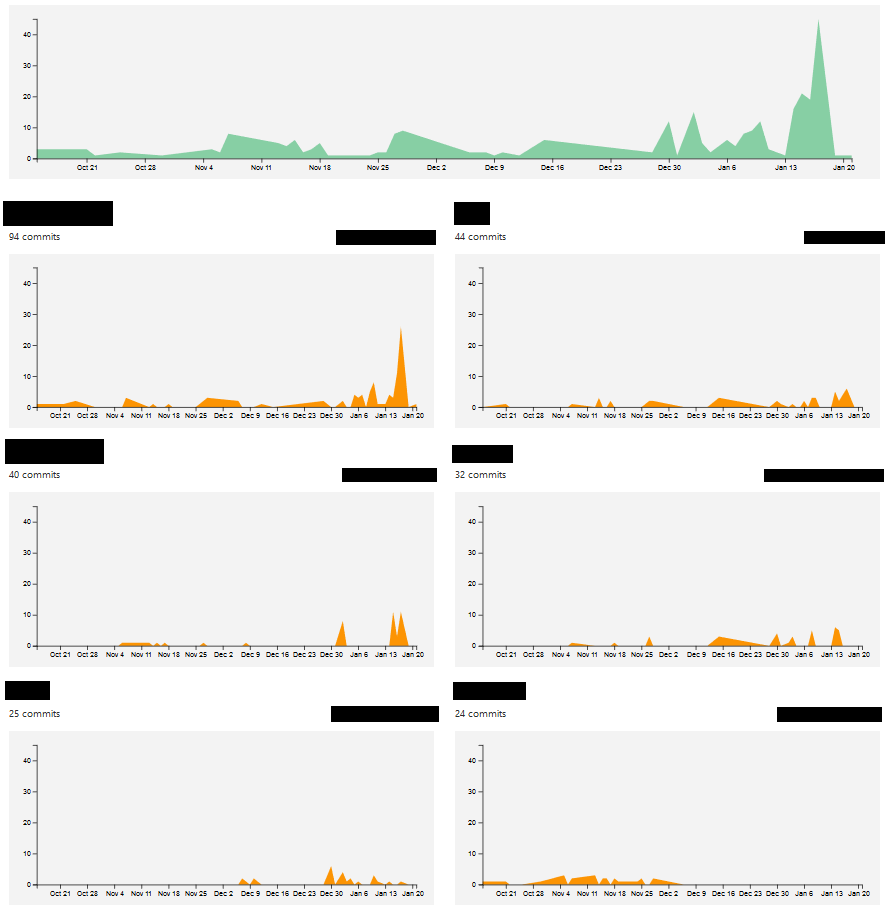
\includegraphics[scale=0.4]{slike/aktivnost.PNG}
			\centering
			\caption{Primjer slike s potpisom}
			\label{fig:promjene}
		\end{figure}
		
		\begin{figure}[H]
			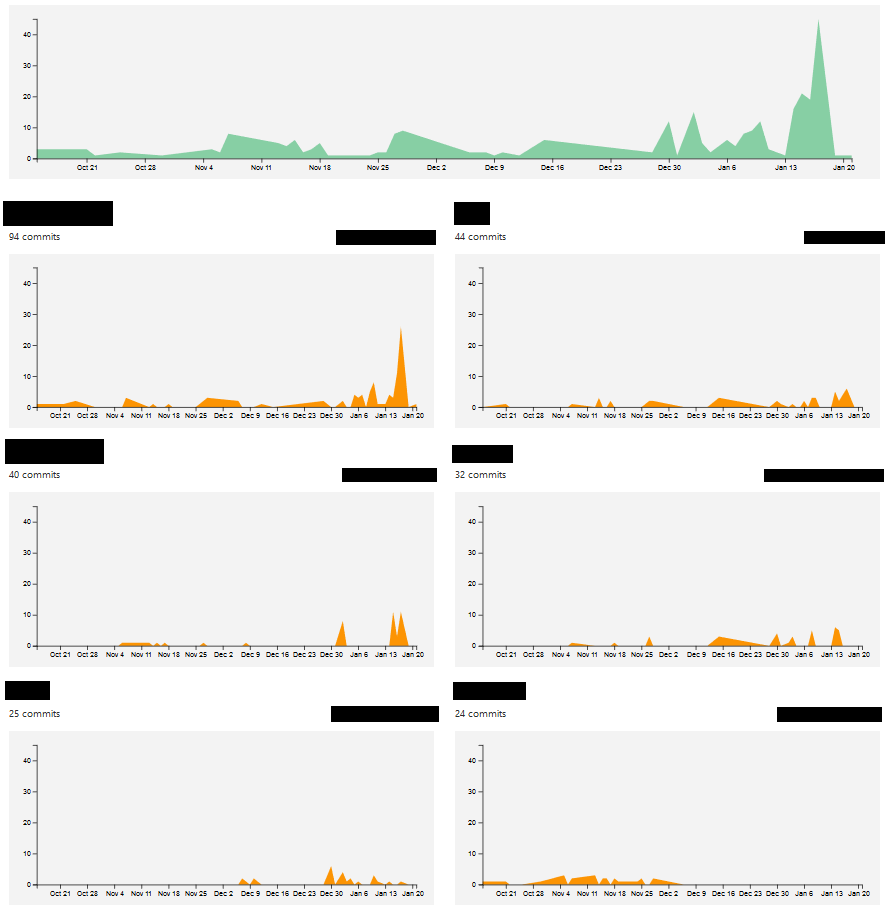
\includegraphics[width=\linewidth]{slike/aktivnost.PNG}
			\caption{Primjer slike s potpisom 2}
			\label{fig:promjene2}
		\end{figure}
		
		
		
		\eject
		
	